
\title{Лекция 1\\Основные положения семантической технологии проектирования интеллектуальных компьютерных систем нового поколения \vspace{-2em}} 
\author[]{Шункевич Д.В.}
\institute[]{Белорусский государственный университет информатики и радиоэлектроники}

\begin{frame}
	\titlepage
\end{frame}

%\begin{frame}{\\Содержание лекции}
%	\vspace{10mm}
%	\topline
%	\justifying
%		Интеллектуальная система, комплексная задача, гибридная интеллектуальная система.
%		Основные положения семантической технологии проектирования интеллектуальных компьютерных систем нового поколения.
%		Основные компоненты указанной технологии.
%		Информационная конструкция, формальный язык, знак, синтаксис, семантика.
%		Семантическая память.
%\end{frame}

\begin{frame}
	\centering
	\Huge
	\textbf{Понятие интеллектуальной компьютерной системы нового поколения}
\end{frame}

\begin{frame}{\\Кибернетическая система}
	\topline
	\justifying

\vspace{10pt}
\begin{SCn}
	\footnotesize
	\scnheader{кибернетическая система}
	\scnidtf{материальная сущность, способная целенаправленно воздействовать на среду своего обитания как минимум для сохранения своей целостности, жизнеспособности, безопасности}
	\scnidtf{система, организация функционирования которой основано на обработке информации о той среде, в которой существует эта система}
	\scnidtf{материальная сущность, способная к активной  целенаправленной деятельности, которая  на определенном уровне развития указанной сущности становится "осмысленной"{}, планируемой, преднамеренной деятельностью}
	\scnidtf{субъект, способный на самостоятельное выполнение некоторых "внутренних"{} и "внешних"{} действий либо порученных извне, либо инициированных самим субъектом}
	\scnidtf{естественная или искусственно созданная система, способная мониторить и анализировать свое состояние и состояние окружающей среды, а также способная достаточно активно воздействовать на собственное состояние и на состояние окружающей среды}
	\scnidtf{система, способная в достаточной степени самостоятельно взаимодействовать со своей средой, решая различные задачи}
	\scnidtf{система, основанная на обработке информации}
\end{SCn}
\end{frame}

\begin{frame}{\\Типология кибернетических систем}
	\topline
	\justifying
	
\begin{SCn}
	\footnotesize
	\scnheader{кибернетическая система}
	\scnrelfrom{разбиение}{Признак естественности или искусственности кибернетических систем}
	\begin{scnindent}
		\begin{scneqtoset}
			\scnitem{естественная кибернетическая система}
			\begin{scnindent}
				\scnidtf{кибернетическая система естественного происхождения}
				\scnsuperset{человек}
			\end{scnindent}
			\scnitem{компьютерная система}
			\begin{scnindent}
				\scnidtf{искусственная кибернетическая система}
				\scnidtf{кибернетическая система искусственного происхождения}
				\scnidtf{технически реализованная кибернетическая система}
			\end{scnindent}
			\scnitem{симбиоз естественных и искусственных кибернетических систем}
			\begin{scnindent}
				\scnidtf{кибернетическая система, в состав которой входят компоненты как естественного, так и
					искусственного происхождения}
				\scnsuperset{сообщество компьютерных систем и людей}
			\end{scnindent}
		\end{scneqtoset}
	\end{scnindent}
\scnsuperset{\scnkeyword{интеллектуальная система}}
\end{SCn}
\end{frame}

\begin{frame}{\\Интеллектуальная компьютерная система}
	\topline
	\justifying
	
\vspace{20pt}
\begin{SCn}
	\footnotesize
	\scnheader{интеллектуальная компьютерная система}
	\scnidtf{интеллектуальная искусственная кибернетическая система}
	\begin{scnrelfromset}{разбиение}
		\scnitem{индивидуальная интеллектуальная компьютерная система}
		\scnitem{интеллектуальный коллектив интеллектуальных компьютерных систем}
		\begin{scnindent}
			\scnidtf{интеллектуальная \textit{многоагентная система}, агенты которой являются \textit{интеллектуальными компьютерными системами}}
			\scntext{примечание}{Не каждый \textit{коллектив интеллектуальных компьютерных систем} может оказаться интеллектуальным, поскольку уровень интеллекта такого коллектива определяется не только уровнем интеллекта его членов, но также и эффективностью (качеством) \uline{их взаимодействия}.}
			\begin{scnrelfromset}{разбиение}
				\scnitem{интеллектуальный коллектив \uline{индивидуальных} интеллектуальных компьютерных систем}
				\scnitem{иерархический интеллектуальный коллектив интеллектуальных компьютерных систем}
			\end{scnrelfromset}
		\end{scnindent}
	\end{scnrelfromset}
\end{SCn}
\end{frame}

\begin{frame}{\\Интеллектуальная система (история понятия)}
	\topline
	\justifying
	\begin{SCn}
		\scnheader{интеллектуальная система} 
		\scnidtf{система, которая способна решать интеллектуальные задачи}

		\scnheader{интеллектуальная задача} 
		\scnidtf{задача, для которой отсутствует известный алгоритм ее решения}

		\scnheader{интеллектуальная система} 
		\scnidtf{система, которая способна обучаться}
	\end{SCn}
\end{frame}

\begin{frame}{\\Интеллектуальная система}
	\topline
	\justifying
	\begin{SCn}
		\scnheader{интеллектуальная система} 
		\scnidtf{система, которая может легко \underline{научиться решать} новые задачи} 
		\begin{scnrelfromset}{важно отличать}
			\scnitem {способность обучаться более \underline{качественному решению} задач \underline{одного ограниченного} класса (как это делают нейросетевые модели)}
			\scnitem {способность обучаться решению задач \underline{разных} классов (с ограничениями или без них)}
		\end{scnrelfromset}
	\end{SCn}
\end{frame}

\begin{frame}{Интеллектуальная компьютерная система нового поколения}
	\topline
	\justifying
	\begin{SCn}
		\footnotesize
		
	\scnheader{интеллектуальные компьютерные системы нового поколения}
	\begin{scnrelfromlist}{предъявляемые требования}
		\scnitem{высокий уровень \textit{интероперабельности}}
		\scnitem{высокий уровень \textit{обучаемости}}
		\scnitem{высокий уровень \textit{гибридности}}
		\scnitem{высокий уровень способности решать \textit{интеллектуальные задачи} (то есть \textit{задачи}, \textit{методы} решения которых и/или требуемая для их решения исходная информация априори неизвестны)}
		\scnitem{высокий уровень \textit{синергетичности}}			
	\end{scnrelfromlist}
	
	\scnheader{интероперабельность\scnsupergroupsign}
	\scnidtf{способность к эффективному (целенаправленному) взаимодействию с другими самостоятельными субъектами}
	\scnidtf{способность работать в коллективе (в команде)}
	\scnidtf{уровень социализации}
	\scnidtf{social skills}
	
	\end{SCn}
\end{frame}


\begin{frame}
	\centering
	\Huge
	\textbf{Технология OSTIS}
\end{frame}

\begin{frame}{\\Комплексная задача}
	\topline
	\justifying
	\begin{SCn}
		\scnheader{комплексная задача}
		\scnidtf{задача, для решения которой необходимо использовать различные виды знаний и различные модели решения задач}
		\scntext{примечание}{Для решения комплексных задач невозможно заранее определить набор моделей решения задач}
		\vspace{5mm}
		\textbf{Примеры комплексных задач:}
		\begin{textitemize}
			\item задача понимания естественных языков, изображений, речевых сообщений
			\item задача планирования поведения интеллектуальных роботов 
			\item задача комплексной автоматизации предприятий
			\item задача адаптивного обучения различным дисциплинам
		\end{textitemize}
	\end{SCn}
\end{frame}

\begin{frame}{\\Гибридная интеллектуальная система}
	\topline
	\justifying
	\vspace{10mm}
	\begin{SCn}
		\scnheader{гибридная интеллектуальная система} 
		\scnidtf{интеллектуальная система, интегрирующая различные виды знаний и различные модели решения задач}
		\scntext{примечание}{ГИС ориентированны на решение комплексных задач}
		\begin{scnrelfromset}{недостатки современного состояния}
				\scnfileitem{монолитность}
				\scnfileitem{ориентированность на решение задачи одного класса (не нескольких различных классов задач)}
				\scnfileitem{требование колоссальных ресурсов (времени) для разработки систем}
				\scnfileitem{невозможность повторного использования компонентов систем для решения других задач (как следствие монолитности)}
		\end{scnrelfromset}
	\end{SCn}
\end{frame}

\begin{frame}{\\Технология OSTIS}
	\topline
	\justifying
	\vspace{10mm}
	\begin{SCn}
		\scnheader{OSTIS}
		\scnidtf{Open Semantic Technology for Intelligent Systems}
		\scnidtf{открытая комплексная технология проектирования совместимых интеллектуальных систем}
		\begin{scnrelfromset}{основные положения}
			\scnfileitem{база знаний OSTIS может описывать \underline{любой вид} знаний}
			\scnfileitem{решатель задач OSTIS основан на многоагентном подходе и позволяет легко \underline{комбинировать любые модели} решения задач}
			\scnfileitem{интерфейс ostis-системы представляет собой подсистему со своей БЗ и решателем задач (также может быть описан с помощью SC-кода)}
			\scnfileitem{использование \underline{универсального} способа представления (кодирования) информации, получившего название SC-код}
		\end{scnrelfromset}
	\end{SCn}
\end{frame}

\begin{frame}{\\}	
	\topline
	\justifying
	\vspace{10mm}
	\begin{SCn}
	\scnheader{OSTIS}
	\begin{scnrelfromset}{достоинства}
		\scnfileitem{унифицированность представления (любая информация представляется \underline{одинаково})}
		\scnfileitem{удобство машинной обработки и восприятия человеком}
		\scnfileitem{любые знания и модели решения задач легко интегрируются в ostis-систему (по принципу plug \& play) и её всегда можно переобучить}
		\scnfileitem{универсальность и совместимость компонентов (повторное использование позволяет сократить время разработки новых компонентов на 40-60\%)}
		\scnfileitem{система описывается с помощью SC-кода, поэтому она может \underline{анализировать себя}, искать в себе ошибки и оптимизировать собственную работу (рефлексивность)}
		\end{scnrelfromset}
	\end{SCn}
\end{frame}

\begin{frame}{\\}
	\topline
	\justifying
	\vspace{10mm}
	\begin{SCn}	
		\scnheader{OSTIS}
		\begin{scnrelfromset}{достоинства}
			\scnfileitem{платформенная независимость (разработка независима от архитектуры компьютера, платформа может быть реализована в программном варианте или в аппаратном)}
			\scnfileitem{параллельная обработка информации}
			\scnfileitem{ostis-система может включать в себя компоненты, разработанные на базе OSTIS, и объединяться с другими системами и интегрировать другие компоненты (с помощью JSON или API)}
			\scnfileitem{производительность ostis-системы не хуже традиционной, а иногда может оказаться лучше за счёт параллельной обработки (при переходе на семантические компьютеры производительность будет ещё выше)}
		\end{scnrelfromset}
	\end{SCn}
\end{frame}
  
\begin{frame}{\\}
	\topline
	\justifying
	\vspace{10mm}
	\begin{SCn}	
		\textbf{Важно понимать:}
			\begin{textitemize}
			\item  {OSTIS -- это не конкретная интеллектуальная система, а \textbf{технология разработки} интеллектуальных систем, каждая из которых будет решать задачи определённого класса}
			\item {ключевые преимущества OSTIS заключаются не в новых функциональных возможностях разрабатываемых систем (большинство функций ostis-систем можно реализовать с помощью традиционных средств), а в том, насколько легко \textbf{модифицировать и развивать} разрабатываемые системы, адаптировать их к новым задачам, а также насколько эффективно можно накапливать и использовать полученные компоненты при разработке новых систем, сокращая при этом время и трудоёмкость их разработки}
			\item {OSTIS -- это способ решения проблемы \textbf{совместимости}, одной из важнейших проблем современных технологий}
			\end{textitemize}
	\end{SCn}
\end{frame}	

\begin{frame}{\\Архитектура ostis-системы}
	\topline
	\justifying
	\vspace{10mm}
	\begin{figure}[H]
		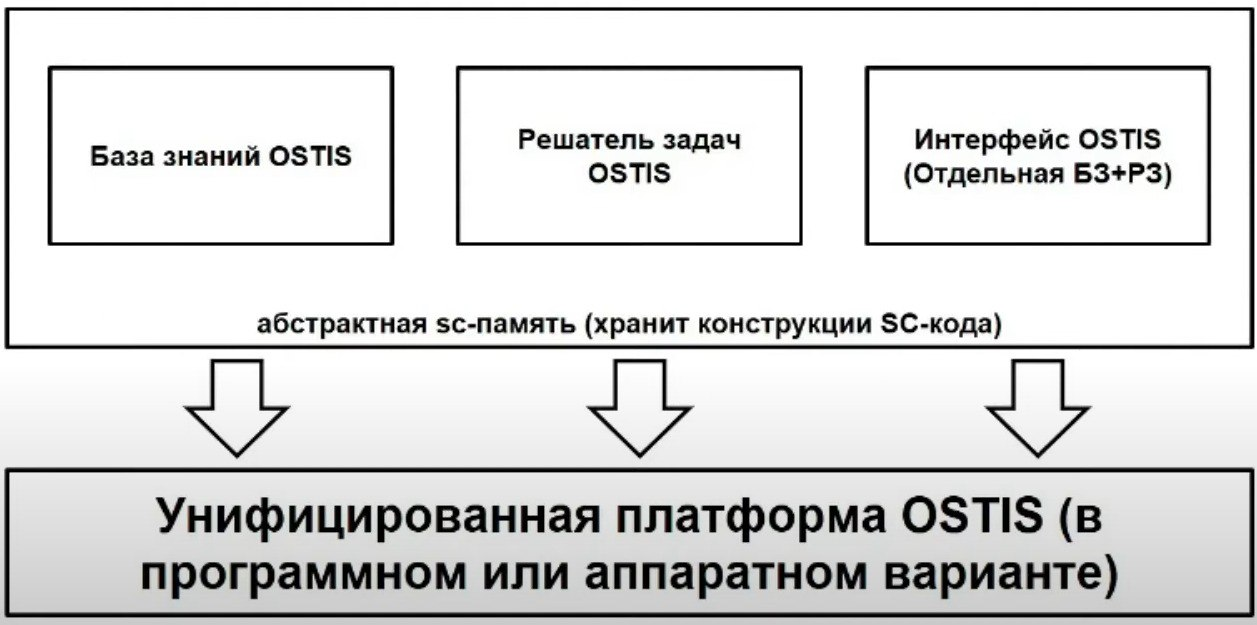
\includegraphics[scale=0.25]{./figures/sd_ostis_basics/scheme.jpeg}
	\end{figure}
\end{frame}

\begin{frame}{\\}
	\topline
	\justifying
	\begin{SCn}	
		\scnheader{база знаний ostis-системы}
		\scnidtf{база знаний, описывающая любой вид знаний, при этом её легко дополнять новыми видами знаний}
		\scnheader{решатель задач ostis-системы}
		\scnidtf{решатель задач, основанный на многоагентном подходе и позволяющий легко интегрировать и комбинировать любые модели решения задач}
		\scnheader{интерфейс ostis-системы}
		\scnidtf{специализированная подсистема ostis-системы со своей базой знаний и решателем задач, предназначенная для общения ostis-системы с внешней средой}
		\scntext{уточнение}{Интерфейс ostis-системы также может быть описан в SC-коде}
	\end{SCn}
\end{frame}

\begin{frame}
	\centering
	\Huge
	\textbf{Информационные конструкции}
\end{frame}

\begin{frame}{\\Информационная конструкция}
	\topline
	\justifying
	\begin{SCn}
		\scnheader{информационная конструкция}
		\scnidtf{конструкция (структура), содержащая некоторые сведения о некоторых сущностях}	
		\scnidtf{информация}
		\scntext{примечание}{Информационная конструкция имеет 
			\begin{textitemize}
				\item форму представления (текст, звук, изображение)
				\item форму структуризации (синтаксис)
				\item смысл (денотационную семантику)
			\end{textitemize}
		}
	\end{SCn}
\end{frame}

\begin{frame}{\\}
	\topline
	\justifying
		\begin{SCn}
		\scnheader{информационная конструкция}
		\begin{scnrelfromset}{разбиение}
			\scnitem{sc-множество}
				\begin{scnindent}
				\scnidtf{внутренняя информационная конструкция ostis-системы, хранимая в её (внутренней) sc-памяти}
				\end{scnindent}
			\scnitem{файл}
				\begin{scnindent}
				\scnidtf{внутреняя информационная конструкция ostis-системы, хранимая в её файловой (внешней) памяти}
				\scntext{примечание}{файл может храниться в памяти другой системы}
				\end{scnindent}
			\scnitem{внешняя информационная конструкция, не являющаяся ни файлом, ни sc-конструкцией}
		\end{scnrelfromset}
	\scnsuperset{дискретная информационная конструкция}
	\end{SCn}
\end{frame}

\begin{frame}{\\Дискретная информационная конструкция}
	\topline
	\justifying
	\begin{SCn}
		\small
		\scnheader{дискретная информационная конструкция}
\scntext{пояснение}{Каждая дискретная информационная конструкция — это информационная конструкция, смысл которой задается:
	\begin{textitemize}
		\item множеством элементов (синтаксически атомарных фрагментов) этой информационной конструкции
		\item алфавитом этих элементов — семейством классов синтаксически эквивалентных элементов информационной конструкции
		\item принадлежностью каждого элемента информационной конструкции соответствующему классу синтаксически эквивалентных элементов информационной конструкции
		\item конфигурацией связей инцидентности между элементами информационной конструкции.
	\end{textitemize}	}
	\end{SCn}
\end{frame}

\begin{frame}{\\}
	\topline
	\justifying
	\begin{SCn}
		\small
		\scnheader{дискретная информационная конструкция}
		\scntext{примечание}{Форма представления элементов дискретной информационной конструкции для анализа её смысла не требует уточнения. Главным является:
		\begin{textitemize}
			\item наличие простой процедуры выделения (сегментации) элементов дискретной информационной конструкции 
			\item наличие простой процедуры установления синтаксической эквивалентности разных элементов дискретной информационной конструкции
			\item наличие простой процедуры установления принадлежности каждого элемента дискретной информационной конструкции соответствующему классу синтаксически эквивалентных элементов (т.е. соответствующему элементу алфавита).
		\end{textitemize}
			}
	\end{SCn}
\end{frame}

\begin{frame}{\\Формальный язык}
	\topline
	\justifying
	\begin{SCn}
		\scnheader{язык}  
		\scnidtf{множество информационных конструкций, построенных по общим синтаксическим и семантическим правилам}
		\begin{scnrelfromset}{разбиение}
			\scnitem{искуственный (построенный) язык}
			\scnitem{формальный язык}
			\scnitem{естественный язык}
		\end{scnrelfromset}
		\scnheader{формальный язык}  
		\scnidtf{язык, в котором значение каждого слова или знака, правила построения предложений и понимания их смысла однозначны}
		\scnidtf{множество конструкций, составленных из некоторого конечного алфавита языка}		
	\end{SCn}
\end{frame}

\begin{frame}{\\Знак}
	\topline
	\justifying
	\begin{SCn}
		\scnheader{знак}
		\scnidtf{фрагмент информационной конструкции, обладающий свойством, \underline{обозначать} некоторую сущность (объект), которая наряду с другими сущностями описывается указанной информационной конструкцией}
		
		\begin{scnrelfromset}{разбиение}
			\scnitem{знак, являющийся элементом \textit{дискретной информационной конструкции}}
			\scnitem{знак, являющийся неатомарным фрагментом \textit{дискретной информационной конструкции}}
		\end{scnrelfromset}
			
	\end{SCn}
\end{frame}

\begin{frame}{\\}
	\topline
	\justifying

Под \textbf{\textit{знаком}} понимается фрагмент \textit{информационной конструкции}, который условно представляет (изображает) некоторую описываемую сущность, которую называют \textbf{\textit{денотатом знака}}.

\bigskip

При этом отсутствие \textit{знака}, обозначающего некоторую сущность, не означает отсутствие самой этой сущности. Это означает только то, что мы даже не догадываемся о ее существовании и, следовательно, не приступили к ее исследованию.

\end{frame}

\begin{frame}{\\Семиотика}
	\topline
	\justifying
	
	\begin{SCn}
\scnheader{семиотика}
\scnidtf{наука о знаках}
\begin{scnrelfromset}{компоненты}
	\scnitem{синтаксис (изучает правильное построение текста)}
	\scnitem{семантика (изучает значение знаков)}
	\scnitem{прагматика (изучает отношение между знаком и субъектом)}
\end{scnrelfromset}

	\end{SCn}
\end{frame}

\begin{frame}{\\Синтаксис и семантика}
	\topline
	\justifying
	\scnheader{синтаксис}
	\scnidtf{наука, изучающая отношения между знаками}
	\scntext{примечание}{Синтаксис переводится как порядок, координация}
	\scnheader{семантика}
	\scnidtf{наука, изучающая отношения между знаками и их значениями}
	\scntext{примечание}{Семантика переводится как обозначение, значение}
\end{frame}


\begin{frame}{\\Семантика}
	\topline
	\justifying
	\vspace{10mm}
	\begin{SCn}
		\scnheader{семантика знака}
		\scnidtf{отношение между знаком и сущностью (значением знака, денотатом), которую он обозначает}
		\begin{figure}[H]
			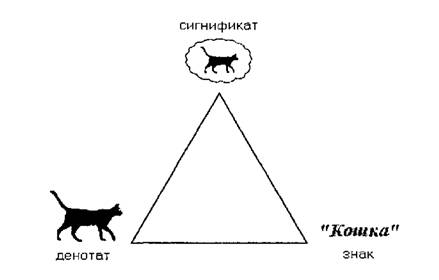
\includegraphics[scale=0.7]{./figures/sd_ostis_basics/sc-code-cat.jpg}
		\end{figure}
	\end{SCn}
\end{frame}

\begin{frame}{\\Семантическая сеть}
	\topline
	\justifying

	\vspace{10mm}

	\begin{SCn}
		\scnheader{семантическая сеть}
		\scnidtf{граф, вершины которого являются знаками некоторых сущностей, а дуги (ребра) -- знаками связей между этими сущностями}
	\end{SCn}
	
	\begin{figure}[H]
		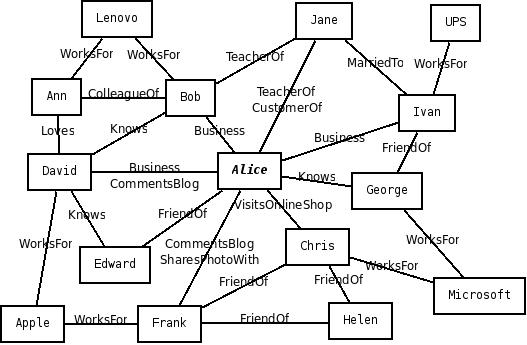
\includegraphics[scale=0.5]{./figures/sd_ostis_basics/sc-code-web.jpg}
		\caption{Пример семантической сети}
	\end{figure}
\end{frame}

\begin{frame}{\\Семантическая память}
	\topline
	\justifying
	\begin{SCn}
		\scnheader{семантическая память}
		\scnidtf{графодинамическая (нелинейная) память}
		\scnidtf{смысловая память, обеспечивающая хранение семантических сетей}
		\scntext{примечание}{Изменение семантической памяти происходит не только путем изменения состояния элементов памяти (вершин графа), но также и изменением конфигурации связей между элементами (ребер или дуг графа)}
	\end{SCn}
\end{frame}


